\documentclass{article}
\usepackage{graphicx}
\usepackage{amsmath}%
\setcounter{MaxMatrixCols}{30}%
\usepackage{amsfonts}%
\usepackage{amssymb}%
\title{IPB Reactor COP Calculation}
%\author{Jin Liu}
%\date{January 25, 2017}
%\date{February 17, 2017}
\setlength\parindent{0pt}
\begin{document}
\maketitle

Definition\\
$Hpdrop:$ \ heater power drop after power deposit to the core in watts\\
$V_{1}:$ voltage RMS measured at the core entrance when $Q$-pulse\\
$V_{2}:$ voltage RMS measured at the core exit when $Q$-pulse\\
$V_{3}:$ voltage RMS measured across the RF termination resistor at the end of the transmission line. The termination resistors are mounted in a copper block that is water cooled . It has constant RF impedance in the freq range we are operating in. With this method we can estimate the pulse current by measuring $V_{3}$ and knowing the $R_{term}$ resistance, $I = V_{3} / R_{term}$ \\
$P:$ applied stimulus power to the core either by $DC$ or $Q$-pulse in watts\\
\\
in $Q$-pulse 

\begin{equation}
P=\frac{(V_{1}-V_{2})*V_{3}}{R_{term}} \label{1}%
\end{equation}
%

$V^{2}=(V_{1}-V_{2})^{2}$ when $Q$-pulse or voltage drop when $DC$ \\
in $DC$


\begin{equation}
P=\frac{V^{2}}{R_{core}} \label{1}%
\end{equation}

$R$ is the resistance of core in $Q$-pulse at a given core temperature as the below:
\begin{equation}
R=\frac{V^{2}}{P}\ [volts^{2}/watts], [volts^{2}/watts]=[ohms]\label{3}%
\end{equation}
%
$M$ is the ratio of Hpdrop vs. applied stimulus power at a given core temperature as the below:
\begin{equation}
M=\frac{Hpdrop}{P}\ \label{4}%
\end{equation}
%
From our experiments, $R$ and $M$ are constants of $Q$-pulse length 100ns and voltage 300v at a given core temperature.\\
\\
Figure 1. shows M vs. temperatures in our two experiments 
\begin{figure}
[h]
\begin{center}
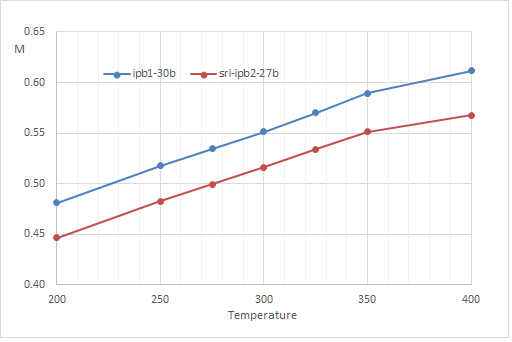
\includegraphics[scale=1]{m.png} 
\caption{M vs. Temperature }%
\end{center}
\end{figure}
From attached plots of $R$ and $M$ vs. temperatures, the error bars defined as the below:
\begin{equation}
ErrorBar=(\Sigma_{i}^{n}{(y_{i}-(\beta_{0}+\beta_{1}*x_{i}))^{2}})^\frac{1}{2}\label{3}%
\end{equation}

$i$ is a single point value of a given temperature, and $n$ is total points of a given temperature. \\


COP Estimation\\
\begin{figure}
[h]
\begin{center}
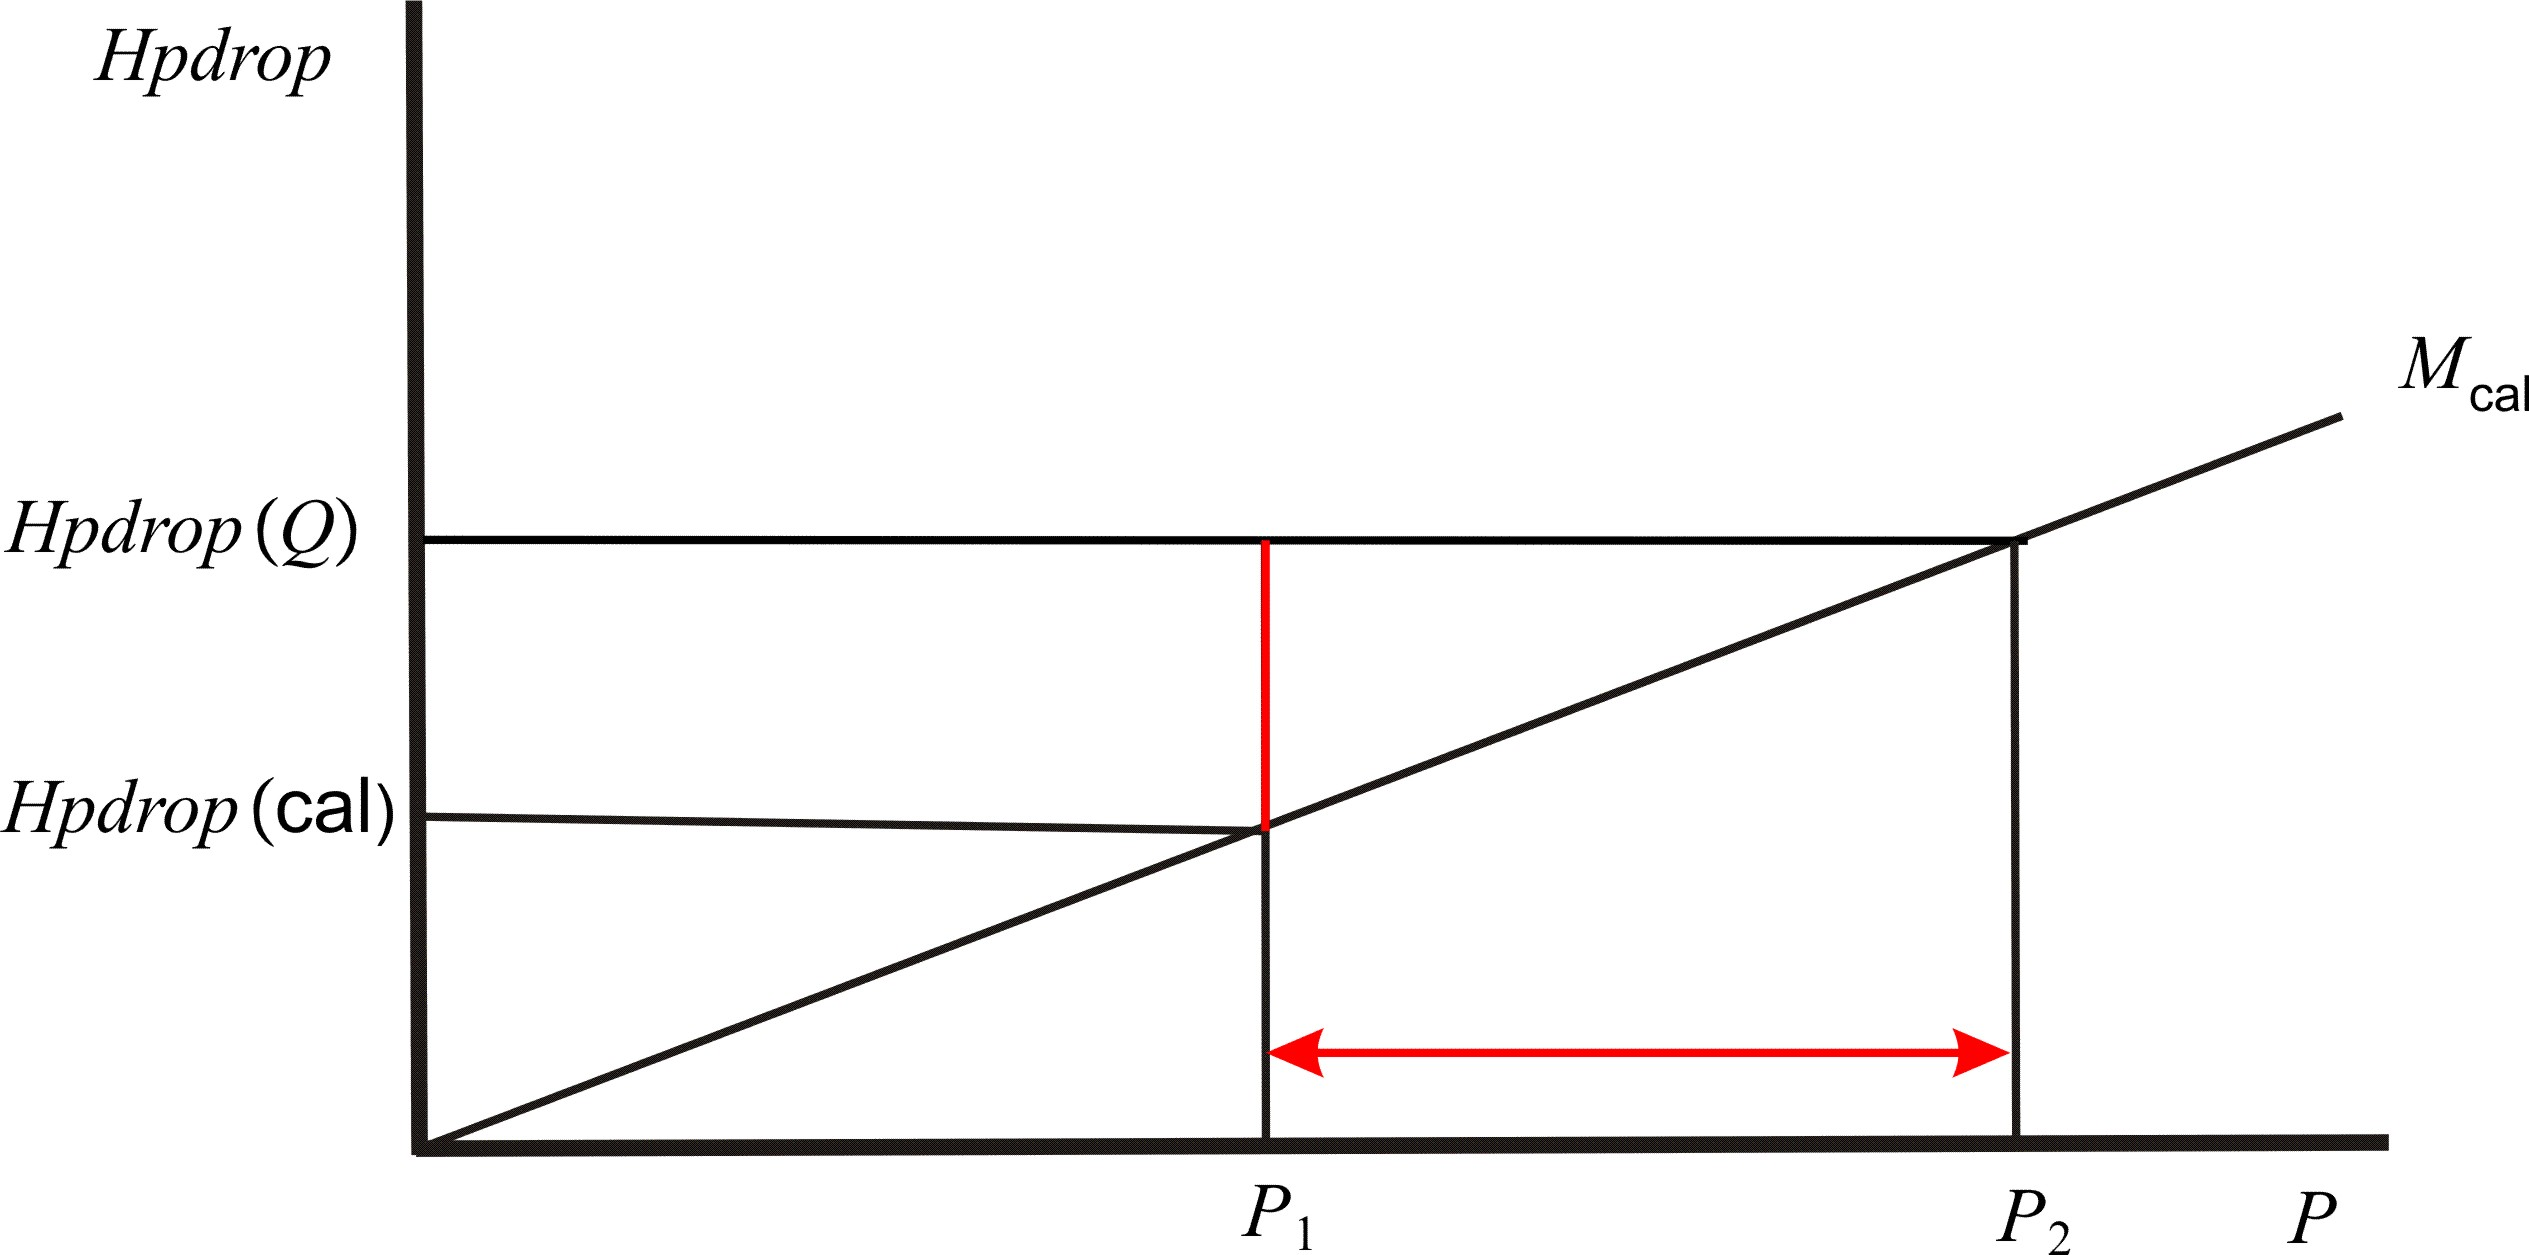
\includegraphics[scale=0.5]{jin3.JPG} 
\caption{Hpdrop vs. P}%
\end{center}
\end{figure}

At a given core temperature\\

From the Figure 2

$P_{1}$ is applied stimulus power from DC or $Q$-pulse

$P_{2}-P_{1}$ is stimulated power gain or LENR (Low Energy Nuclear Reaction) Power \\

$COP$ is Coefficient Of Performance\\
\begin{equation}
P_{2} = \frac{Hpdrop(Q)}{M_{cal}}
\end{equation}

\begin{equation}
COP=1+\frac{P_{2}-P_{1}}{P_{1}}=\frac{P_{2}}{P_{1}}=\frac{Hpdrop(Q)}{M_{cal}*P_{1}} \label{4}%
\end{equation}


COP calculation of ipb1-30b and sri-ipb2-27b are in Figure 3 and Figure 4.
\begin{figure}
[h]
%\begin{top}
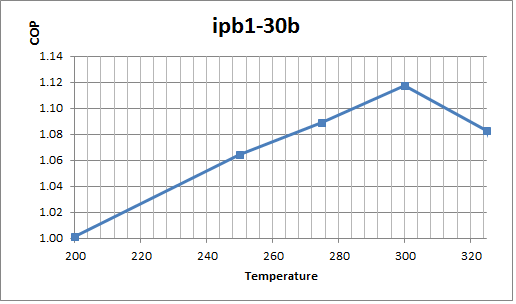
\includegraphics[scale=1.0]{ipb-30b.png} 
\caption{COP vs. temperature of ipb1-30b}%
%\end{top}
\end{figure}

\begin{figure}
%[h]
%\begin{bottom}
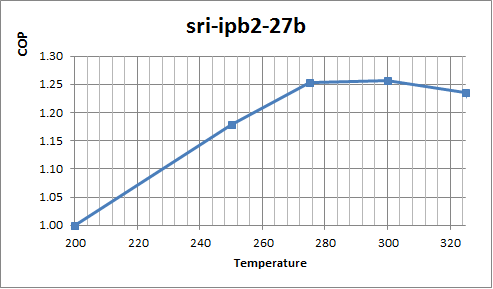
\includegraphics[scale=1.0]{sri-ipb2-27b.png} 
\caption{COP vs. temperature of sri-ipb2-27b}%
%\end{bottom}
\end{figure} 


\end{document}